\section{Performance analysis}

We approached the performance analysis by designing a simple data schema which consist of a one-to-many relation, many-to-many relation, and a reverse relation.
To easier understand it and discuss it, we assign to entities in the schema meaningful names of a simple blog application.
Figure \ref{schema} shows the entities and relations between them.

\begin{figure}[!h]
\centering
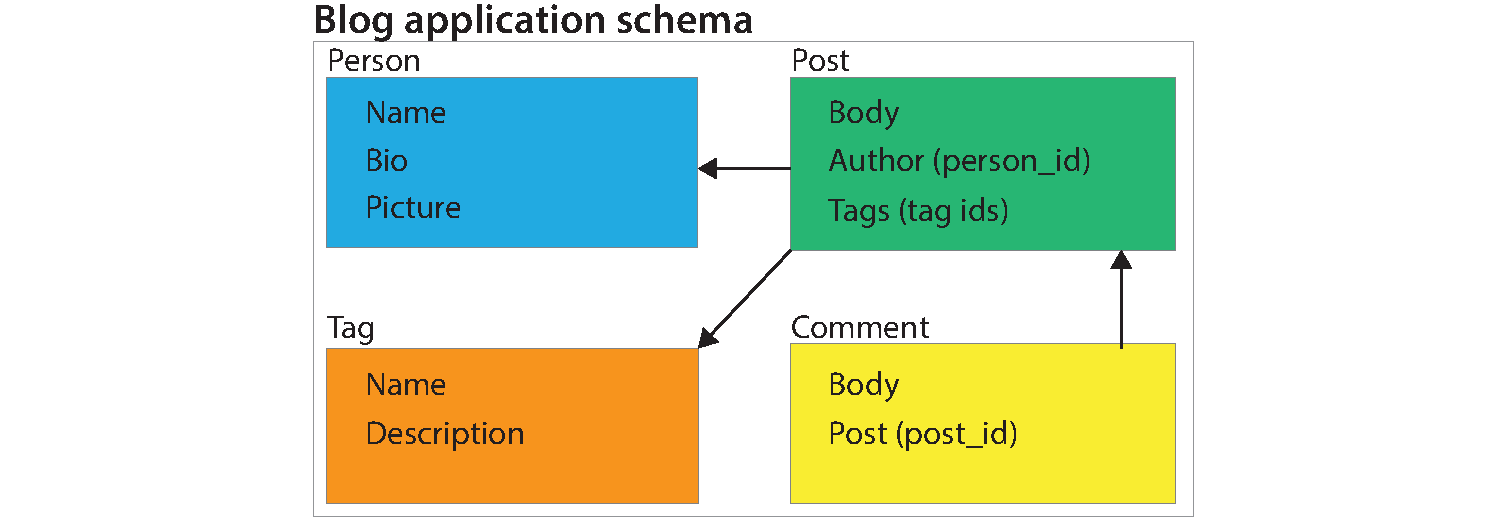
\includegraphics[width=0.9\columnwidth]{schema}
\caption{A blog post is the main entity we are querying. It has one-to-many \emph{author} relation to person entity and many-to-many \emph{tags} relation to tag entity. Comment entity has a one-to-many \emph{post} relation to the post entity, for which this relation is a reverse relation where we are interested in all comments made for a given post.}
\label{schema}
\end{figure}

To measure performance we decided to use a query which uses all relatons in the schema.
By querying for a blog post document, in addition to the post data itself, we want to get:
\begin{itemize}
\item name and picture of the author
\item name and description of all tags of the blog post
\item body of all blog post's comments
\end{itemize}

The concrete query we used is as follows: based on a string tag name, obtain all blog posts which are tagged with that tag, and for each blog post above mentioned additional data have to be available.

To be able to compare the measurements we implemented this schema and query in multiple systems:
\begin{itemize}
\item using PostgreSQL relational DBMS with low-level queries in Python
\item using PostgreSQL relational DBMS with high-level queries in Django, a Python based web framework
\item using MongoDB with low-level queries in Python
\item using MongoDB with high-level queries in Meteor
\item using MongoDB with PeerDB in Meteor
\item using MongoDB with PeerDB in Python
\end{itemize}

The motivation was to measure both low-level and high-level database interfaces to be able to compare difference between using a high-level web framework and not. To measure both traditional relational DBMS and NoSQL one. And of course to see how it works when using PeerDB and when not.

\begin{table}
  \small
  \begin{center}
  \begin{tabular}{|l|l|l|l|}
    %\hline
    \hline
    Entity & Number of documents\\
    \hline
    Person & 100 \\
    Tags & 100 \\ 
    Posts & 1000 \\ 
    Comments & 10000 \\ 
    \hline

  \end{tabular}
  \end{center}
  \caption{Basic number of documents used in the benchmark.}
  \label{numbers}
\end{table}

\begin{table}
  \small
  \begin{center}
  \begin{tabular}{|l|l|l|l|}
    %\hline
    \hline
    Field & Size in bytes\\
    \hline
    Person name & 11 \\
    Person bio & 1000 \\ 
    Person picture & 10 \\ 
    Tag name & 11 \\ 
    Tag description & 10 \\
    Post body & 1000 \\
    Comment body & 10 \\
    \hline

  \end{tabular}
  \end{center}
  \caption{Basic size of fields in documents used in the benchmark.}
  \label{sizes}
\end{table}

Basic number of tags per post was 10.
We uniformly distributed all comments across all blog posts. For future work we could consider using a long-tailed distribution.

We scaled this basic numbers to vary:
\begin{itemize}
\item number of documents, we used multiplication factors 1, 2, 4, 6, 8, 10
\item size of person picture, tag description, and comment body fields in documents, we used multiplication factors 1, 10, 100, 1000, 10000, 100000
\end{itemize}

When varying one dimension we kept the other at its basic value.

In addition, for two PeerDB based systems (Meteor and Python) we additionally vary how many PeerDB instances are observing and handling the changes in the database, running all above variations on 1, 2, 4, 6, 8 and 10 instances.
